\documentclass[aspectratio=169,11pt]{beamer}
\usepackage[T1]{fontenc}
\usepackage{tgpagella}
\usepackage{amsmath,amssymb}
\usepackage{tikz}
\usetikzlibrary{arrows.meta,positioning,calc}
\usepackage{graphicx}

\definecolor{paper}{HTML}{FBF9F4}
\definecolor{ink}{HTML}{23211E}
\definecolor{ox}{HTML}{8C2F24}
\definecolor{slate}{HTML}{4A6274}
\definecolor{hair}{HTML}{D6CFBF}
\definecolor{faded}{HTML}{8A8375}

\setbeamercolor{normal text}{fg=ink,bg=paper}
\setbeamercolor{structure}{fg=ox}
\setbeamertemplate{navigation symbols}{}
\setbeamertemplate{background canvas}{\color{paper}\vrule width\paperwidth height\paperheight}
\setbeamerfont{frametitle}{size=\large,series=\bfseries}
\setbeamertemplate{frametitle}{%
  \vspace*{2.5mm}%
  {\color{ox}\footnotesize\scshape\insertframenumber\quad}%
  {\color{ink}\large\bfseries\insertframetitle}\\[-1mm]
  {\color{hair}\rule{\textwidth}{0.4pt}}}
\setbeamersize{text margin left=13mm,text margin right=13mm}
\setbeamertemplate{itemize item}{\color{ox}\raisebox{0.1em}{\scriptsize$\bullet$}}
\setbeamertemplate{itemize subitem}{\color{faded}\raisebox{0.1em}{\scriptsize$\circ$}}

\newcommand{\C}{\mathbb{C}}
\newcommand{\ip}[2]{\langle #1|#2\rangle}
\newcommand{\aside}[1]{{\color{faded}\small #1}}
\newcommand{\bigclaim}[1]{{\Large\bfseries #1\par}}
\newcommand{\wideaside}[1]{\begin{center}\parbox{0.90\textwidth}{\centering\aside{#1}}\end{center}}
\newcommand{\interlude}[2]{%
  \begin{frame}[plain]
    \vspace*{22mm}
    \begin{center}
      \begin{minipage}{0.86\textwidth}
        \centering
        {\color{ox}\rule{18mm}{1.2pt}}\\[6mm]
        {\LARGE\itshape #1\par}\vspace{5mm}
        {\color{faded}\normalsize #2\par}
      \end{minipage}
    \end{center}
  \end{frame}}
\setbeamertemplate{footline}{}

\begin{document}

% ---------------------------------------------------------------- 1 title
\begin{frame}[plain]
  \vspace*{4mm}
  \begin{columns}[c]
  \begin{column}{0.60\textwidth}
    {\color{ox}\footnotesize\scshape a problem in dimension six}\\[3mm]
    {\color{ink}\fontsize{30}{34}\selectfont\bfseries Three mutually\\[1mm] unbiased bases\\[1mm] in $\C^6$\par}
    \vspace{5mm}
    {\color{faded}\normalsize A computer-assisted answer,\\
    and an honest account of what it rests on.}
  \end{column}
  \begin{column}{0.36\textwidth}
    \centering
    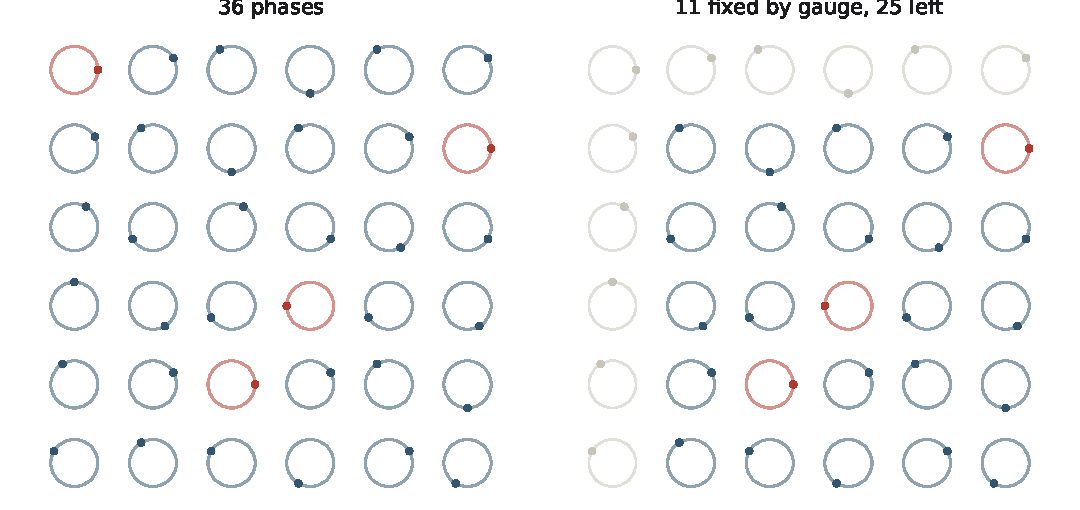
\includegraphics[width=\textwidth]{figs/fig_phases.pdf}
  \end{column}
  \end{columns}
  \vfill
  {\color{faded}\footnotesize Mathathon working group\hfill November 2026}
\end{frame}

% ---------------------------------------------------------------- 2 what unbiased means
\begin{frame}{What ``unbiased'' means}
  \vspace{2mm}
  \begin{columns}[c]
  \begin{column}{0.5\textwidth}
    {\large Two bases are unbiased when a measurement in one tells you \emph{nothing} about the
    outcome in the other.}
    \vspace{4mm}

    {\normalsize Concretely: every overlap has size $1/\sqrt6$, so every entry of the $6\times6$
    table of overlaps is $1/6$ in absolute value squared.}
    \vspace{4mm}

    \aside{Maximally incompatible. Learn the answer to one question, learn nothing about the other.}
  \end{column}
  \begin{column}{0.46\textwidth}
    \centering
    \scalebox{0.80}{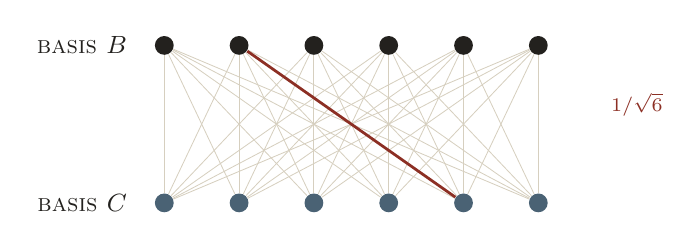
\begin{tikzpicture}[scale=1.0]
      \foreach \i in {0,...,5}{
        \node[circle,fill=ink,inner sep=2.4pt] (a\i) at (\i*0.95,2.0) {};
        \node[circle,fill=slate,inner sep=2.4pt] (b\i) at (\i*0.95,0) {};}
      \foreach \i in {0,...,5}{\foreach \j in {0,...,5}{
        \draw[hair,line width=0.3pt] (a\i)--(b\j);}}
      \draw[ox,line width=1.0pt] (a1)--(b4);
      \node[ox,font=\small,anchor=west] at (5.55,1.25) {\scriptsize$1/\sqrt6$};
      \node[font=\small\scshape,anchor=east,color=ink] at (-0.35,2.0) {basis $B$};
      \node[font=\small\scshape,anchor=east,color=ink] at (-0.35,0.0) {basis $C$};
    \end{tikzpicture}}
  \end{column}
  \end{columns}
\end{frame}

% ---------------------------------------------------------------- 3 the question
\interlude{How many such bases
fit in $\C^6$?}{Three, says a 76-page preprint from last September.
Not six, not four.}

\begin{frame}{Six is the awkward dimension}
  \vspace{1mm}
  \begin{columns}[c]
  \begin{column}{0.52\textwidth}
    When the dimension is a prime power you get a complete set: $d+1$ bases, no slack, a clean
    algebraic construction.

    \vspace{4mm}
    Six is not a prime power. The construction gives nothing, and for twenty years the best anyone
    could say was $3\le N(6)\le 7$.

    \vspace{4mm}
    \aside{The obstruction here is not arithmetic. It is the shape of a $45$-dimensional torus of
    phases, and the claim is that a finite computation can cut it down to points.}
  \end{column}
  \begin{column}{0.44\textwidth}
    \centering
    \scalebox{0.74}{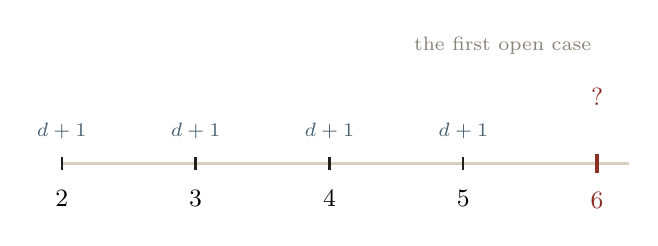
\begin{tikzpicture}[font=\small]
      \draw[hair,line width=0.8pt] (0,0)--(7.2,0);
      \foreach \x/\d/\l in {0/2/{$d+1$},1.7/3/{$d+1$},3.4/4/{$d+1$},5.1/5/{$d+1$}}{
        \draw[ink,line width=0.8pt] (\x,0)++(0,-0.08)--++(0,0.16);
        \node[below=3pt] at (\x,-0.12) {$\d$};
        \node[above=2pt,font=\scriptsize,color=slate] at (\x,0.12) {\l};}
      \draw[ox,line width=1.4pt] (6.8,0)++(0,-0.12)--++(0,0.24);
      \node[below=3pt,color=ox] at (6.8,-0.14) {$6$};
      \node[above=9pt,font=\small,color=ox,align=center] at (6.8,0.3) {?};
      \node[above=26pt,font=\scriptsize,color=faded,align=center] at (5.6,0.35)
        {the first open case};
    \end{tikzpicture}}
  \end{column}
  \end{columns}
\end{frame}

% ---------------------------------------------------------------- 4 the trick
\begin{frame}{The move that makes it computable}
  \vspace{1mm}
  Fix the first basis to be the coordinate basis. Then a second basis is nothing but a $6\times6$
  matrix of phases satisfying one quadratic equation, $HH^{*}=6I$ --- a \emph{complex Hadamard
  matrix}.

  \vspace{3mm}
  Rephasing rows and columns is free, and it removes $11$ of the $36$ phases.
  \textbf{Twenty-five phases decide everything.}

  \vspace{2mm}
  \begin{columns}[c]
  \begin{column}{0.42\textwidth}
    \centering
    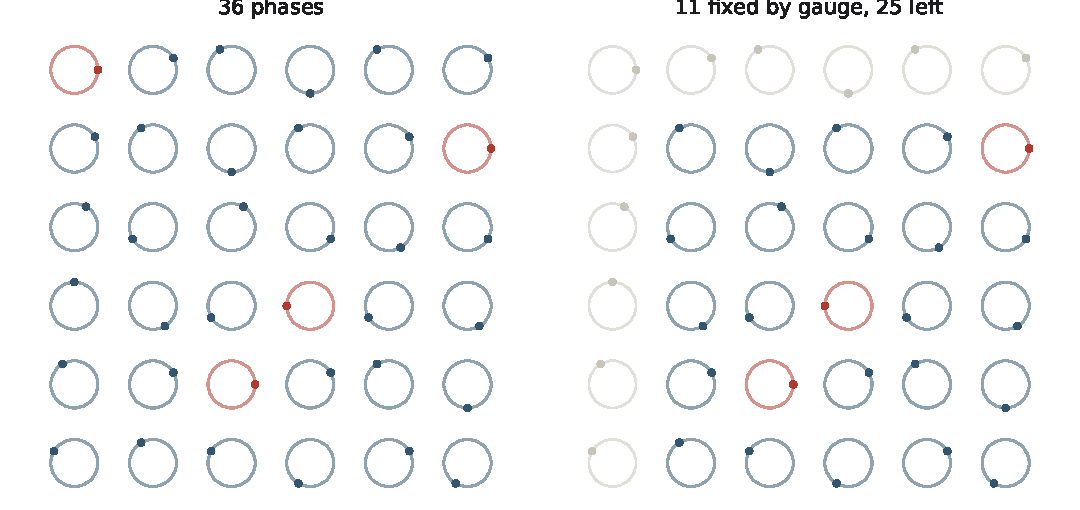
\includegraphics[width=0.9\textwidth]{figs/fig_phases.pdf}
  \end{column}
  \begin{column}{0.54\textwidth}
    \aside{Each dot is one phase, drawn on its own circle. Grey entries are fixed by the gauge.
    What is left is a $25$-dimensional landscape --- and the theorem has to exclude two further
    bases at \emph{every} point of it, not just on a nice family.}

    \vspace{3mm}
    {\normalsize That quantifier is the part that had not been done before.}
  \end{column}
  \end{columns}
\end{frame}

% ---------------------------------------------------------------- 5 the ladder
\begin{frame}{Five steps, each one a cover}
  \vspace{6mm}
  \begin{center}
  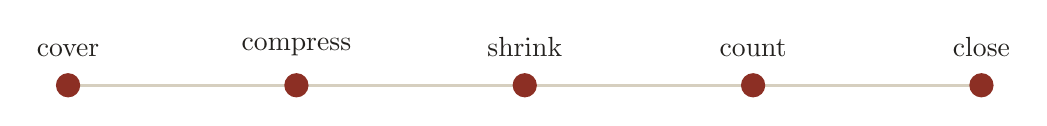
\begin{tikzpicture}[font=\small,
    st/.style={circle,fill=ox,inner sep=3.1pt},
    lb/.style={font=\normalsize,color=ink},
    gl/.style={font=\scriptsize,color=faded,align=center,text width=2.6cm}]
    \draw[hair,line width=1pt] (0.9,0)--(12.5,0);
    \foreach \x/\w in {0.9/cover, 3.8/compress, 6.7/shrink, 9.6/count, 12.5/close}{
      \node[st] at (\x,0) {};
      \node[lb,above=7pt] at (\x,0) {\w};}
  \end{tikzpicture}
  \end{center}
  \vspace{8mm}
  \begin{center}
    {\normalsize Every arrow keeps \emph{everything} the previous step could have produced.\\
    Bin, then compress, then shrink, then count, then close.}
  \end{center}
\end{frame}

% ---------------------------------------------------------------- 6 cover
\begin{frame}{Cover the circle}
  \vspace{1mm}
  \begin{columns}[c]
  \begin{column}{0.52\textwidth}
    {\large Only nine phases of a Hadamard actually need covering. Put a grid of $112$ bins on each
    and ask, bin pair by bin pair, whether an exact solution could live inside.}

    \vspace{5mm}
    {\color{faded}\small bin pairs examined}\\[-1mm]
    {\Large $151{,}744{,}086$}\\[2mm]
    {\color{faded}\small survivors, kept as balls}\\[-1mm]
    {\Large $249{,}878$}

    \vspace{5mm}
    \aside{A pair dies only when a necessary inequality fails on the whole box --- a gap bound, a
    Taylor test on two vanishing sums, a shared coordinate. No sampling, no hope.}
  \end{column}
  \begin{column}{0.44\textwidth}
    \centering
    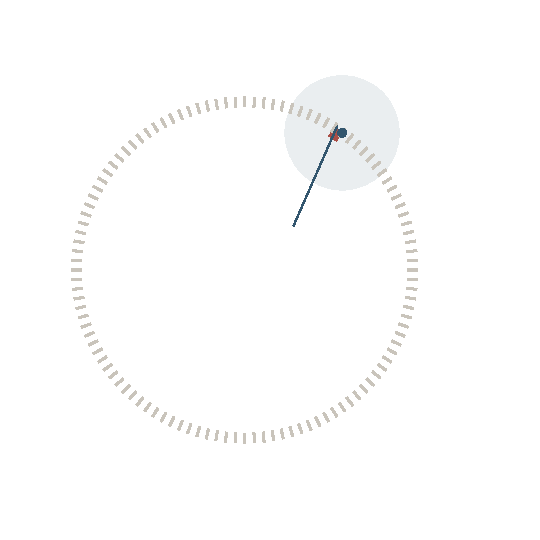
\includegraphics[width=0.78\textwidth]{figs/fig_cover.pdf}\\[2mm]
    {\color{faded}\scriptsize one bin, and the ball of radius $0.032$ cycles that covers it\\
    (drawn much larger than life)}
  \end{column}
  \end{columns}
\end{frame}

% ---------------------------------------------------------------- 7 compress
\begin{frame}{A $6\times6$ unknown becomes a point of $U(2)$}
  \vspace{1mm}
  \begin{columns}[c]
  \begin{column}{0.52\textwidth}
    Split the matrix into a $2\times2$ corner and a $4\times4$ block. At the centre of a seed ball the
    two off-diagonal blocks have rank two, so their kernels are fixed for the whole ball.

    \vspace{3mm}
    Squeeze the unknown $4\times4$ block between those kernels. What comes out is a matrix that is
    within $p$ of $\sqrt6$ times a \emph{unitary}, so every completion of the seed is a point of
    $U(2)$ --- four angles, one square.

    \vspace{3mm}
    \aside{This is the neat device in the paper: an infinite-dimensional-looking condition
    collapses onto a compact four-parameter chart.}
  \end{column}
  \begin{column}{0.42\textwidth}
    \centering
    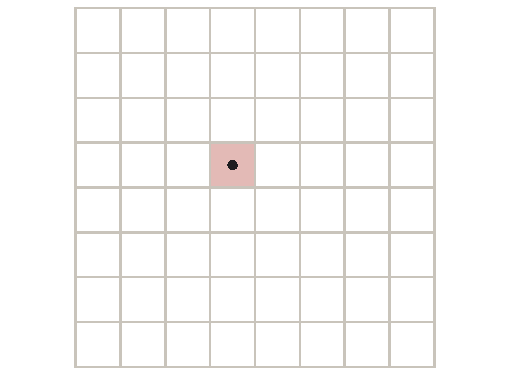
\includegraphics[width=0.86\textwidth]{figs/fig_chart.pdf}\\[1mm]
    {\color{faded}\scriptsize cut $U(2)$ into cells; follow the one the completion lands in}
  \end{column}
  \end{columns}
\end{frame}

% ---------------------------------------------------------------- 8 shrink
\begin{frame}{Shrink, with a witness}
  \vspace{2mm}
  {\large A ball is only useful if you can make it small. Each centre carries a numerical frame and
  a few constants that together bound how far an exact matrix can sit from the centre --- and that
  bound can be iterated.}

  \vspace{6mm}
  \begin{center}
  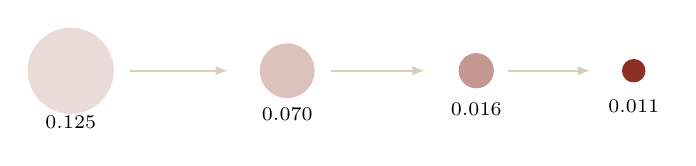
\begin{tikzpicture}[font=\small]
    \node[circle,fill=ox!18,inner sep=11pt] (a) at (0,0) {};
    \node[font=\scriptsize,below=13pt] at (a) {$0.125$};
    \draw[-{Latex[length=1.6mm]},hair,line width=0.8pt] (0.75,0)--(2.0,0);
    \node[circle,fill=ox!30,inner sep=7pt] (b) at (2.75,0) {};
    \node[font=\scriptsize,below=10pt] at (b) {$0.070$};
    \draw[-{Latex[length=1.6mm]},hair,line width=0.8pt] (3.3,0)--(4.5,0);
    \node[circle,fill=ox!50,inner sep=4.5pt] (c) at (5.15,0) {};
    \node[font=\scriptsize,below=8pt] at (c) {$0.016$};
    \draw[-{Latex[length=1.6mm]},hair,line width=0.8pt] (5.55,0)--(6.6,0);
    \node[circle,fill=ox,inner sep=3pt] (d) at (7.15,0) {};
    \node[font=\scriptsize,below=7pt] at (d) {$0.011$};
  \end{tikzpicture}
  \end{center}
  \vspace{4mm}
  \wideaside{Three passes. A parent that refuses to shrink stays on the books as an
  obligation --- it never counts as a pass.}
\end{frame}

% ---------------------------------------------------------------- 9 count
\begin{frame}{Inside the last ball, it is a counting problem}
  \vspace{1mm}
  \begin{columns}[c]
  \begin{column}{0.5\textwidth}
    Every vector unbiased to the first basis is fixed by five phases. Bin them, cluster the survivors
    into vector balls, and draw two graphs: orthogonality not yet excluded, unbiasedness not yet
    excluded.

    \vspace{3mm}
    Two further bases would be two hexagons of orthogonal pairs with \emph{all thirty-six} cross
    edges present in the second graph.

    \vspace{3mm}
    {\large That pattern does not exist. The ball is out.}
  \end{column}
  \begin{column}{0.46\textwidth}
    \centering
    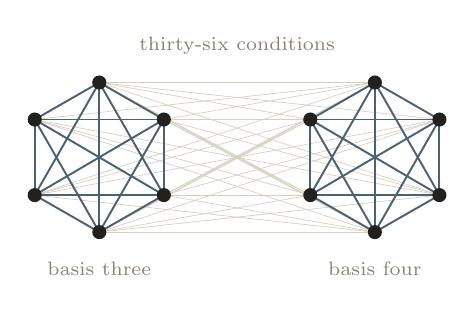
\begin{tikzpicture}[font=\scriptsize,dot/.style={circle,fill=ink,inner sep=1.8pt}]
      \foreach \k/\dx in {L/0,R/3.5}{
        \coordinate (\k1) at (\dx+0,0.95); \coordinate (\k2) at (\dx-0.82,0.48);
        \coordinate (\k3) at (\dx-0.82,-0.48); \coordinate (\k4) at (\dx+0,-0.95);
        \coordinate (\k5) at (\dx+0.82,-0.48); \coordinate (\k6) at (\dx+0.82,0.48);}
      \foreach \i in {1,...,6}{\foreach \j in {1,...,6}{\draw[hair,line width=0.25pt] (L\i)--(R\j);}}
      \foreach \k in {L,R}{\foreach \i/\j in {1/2,1/3,1/4,1/5,1/6,2/3,2/4,2/5,2/6,3/4,3/5,3/6,4/5,4/6,5/6}{
        \draw[slate,line width=0.7pt] (\k\i)--(\k\j);}}
      \foreach \k in {L,R}{\foreach \i in {1,...,6}{\node[dot] at (\k\i) {};}}
      \node[color=faded] at (1.75,1.42) {thirty-six conditions};
      \node[color=faded] at (0,-1.42) {basis three};
      \node[color=faded] at (3.5,-1.42) {basis four};
    \end{tikzpicture}
  \end{column}
  \end{columns}
\end{frame}

% ---------------------------------------------------------------- 10 video
\begin{frame}[plain]
  \begin{columns}[c]
  \begin{column}{0.42\textwidth}
    \vspace*{4mm}
    {\color{ox}\footnotesize\scshape the code, running}\\[3mm]
    {\Large\bfseries Forty-five seconds\\ of the real thing}\\[3mm]
    {\color{faded}\small The exact integer tests that throw out every candidate for a fourth basis
    on one worked pair. No cuts, no voice-over.}

    \vspace{4mm}
    {\color{faded}\scriptsize\texttt{examples/step4\_example.py}\\[1mm]
    \texttt{slides/video/stageC-demo.mp4}}
  \end{column}
  \begin{column}{0.56\textwidth}
    \centering
    \begin{tikzpicture}
      \node[inner sep=0] (p) {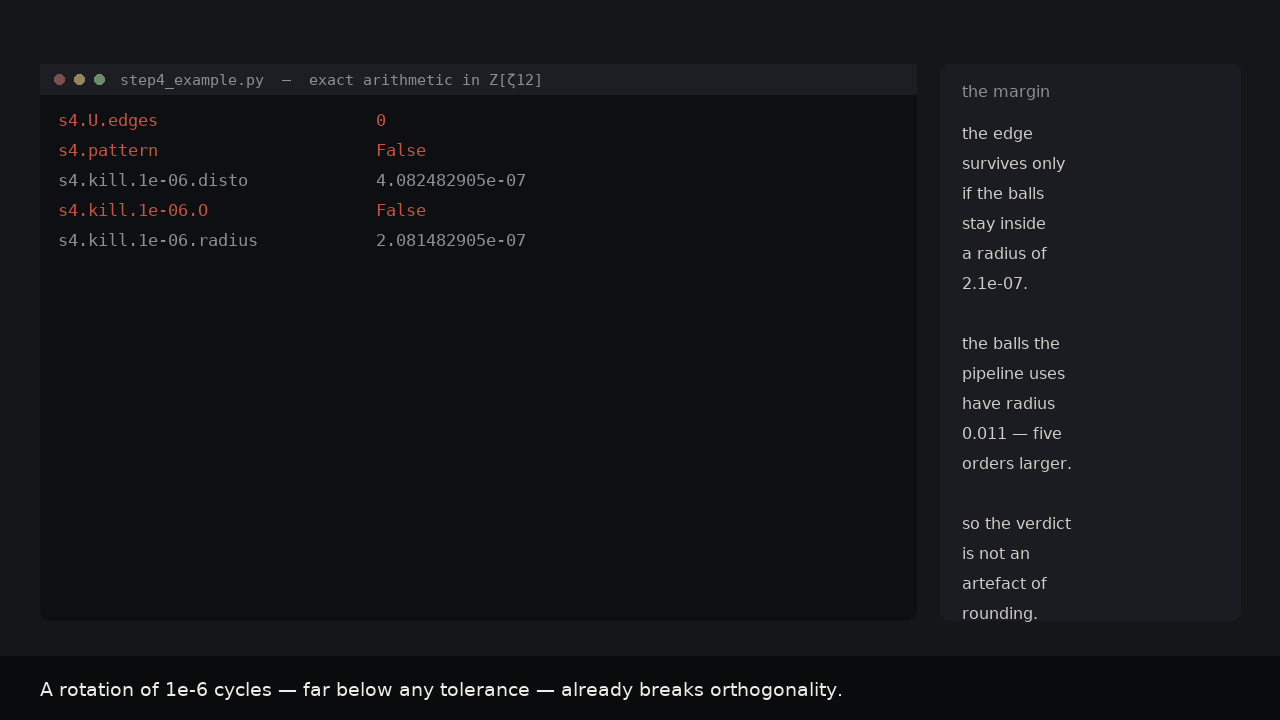
\includegraphics[width=\textwidth]{video/poster.png}};
      \fill[white,opacity=0.9] ($(p.center)+(-5mm,0)$) -- ($(p.center)+(11mm,7mm)$) -- ($(p.center)+(11mm,-7mm)$) -- cycle;
    \end{tikzpicture}
  \end{column}
  \end{columns}
\end{frame}

% ---------------------------------------------------------------- 11 fine print
\begin{frame}{What this proof actually assumes}
  \vspace{2mm}
  The mathematics is a colleciton of necessary conditions. That the search \emph{closes} is not
  proved --- it is observed. Three things have to be true for the theorem to stand.

  \vspace{6mm}
  \begin{columns}[T]
  \begin{column}{0.31\textwidth}
    {\color{ox}\scshape the arithmetic}\\[1mm]
    {\footnotesize Everything is binary64, with twenty pages of one-sided error budgets and a build
    tuned to one machine. Change the compiler and you change the experiment.}
  \end{column}
  \begin{column}{0.31\textwidth}
    {\color{ox}\scshape the run}\\[1mm]
    {\footnotesize Seven programs, a hundred invocations, seventy-five minutes, records archived
    with hashes. The hypothesis is an event, not an inequality.}
  \end{column}
  \begin{column}{0.31\textwidth}
    {\color{ox}\scshape the code}\\[1mm]
    {\footnotesize That the programs do what the lemmas say. The paper says so in prose; no code
    appears in it.}
  \end{column}
  \end{columns}
  \vspace{8mm}
  \wideaside{\footnotesize One rule survives all three: propose cheaply, certify
  separately, and let anything uncertified stay \emph{unresolved}. Unresolved is never a negative.}
\end{frame}

% ---------------------------------------------------------------- 12 what we checked
\begin{frame}{What we have actually checked}
  \vspace{3mm}
  \begin{columns}[c]
  \begin{column}{0.33\textwidth}
    {\color{ox}\fontsize{26}{28}\selectfont\bfseries 249\,878}\\[1mm]
    centres, reproduced byte for byte by a clean-room implementation.\\
    \aside{Same file, same hash, 400.8 seconds against the published 401.8.}
  \end{column}
  \begin{column}{0.33\textwidth}
    {\color{ox}\fontsize{26}{28}\selectfont\bfseries 151\,744\,086}\\[1mm]
    seed-cover records re-checked, with zero missing pairs and zero undecided comparisons.
  \end{column}
  \begin{column}{0.33\textwidth}
    {\color{ox}\fontsize{26}{28}\selectfont\bfseries 269\,403}\\[1mm]
    basic pair predicates recomputed exactly or outwards, on four complete batches ---
    $133\,944$ certified exclusions, no interval left undecided.
  \end{column}
  \end{columns}
  \vspace{7mm}
  \wideaside{Also: one Stage-B parent covered end to end by two arithmetic routes, twenty
  Stage-A directional certificates, thirty-six Root witnesses, and a Lean-checked assembly of the
  six interfaces --- conditional on the rest.}
\end{frame}

% ---------------------------------------------------------------- 13 k=0
\begin{frame}{You cannot even add one vector}
  \vspace{1mm}
  A fourth basis needs six vectors unbiased to all three existing bases. It turns out that
  \emph{none} exists.

  \vspace{4mm}
  \begin{columns}[c]
  \begin{column}{0.54\textwidth}
    {\small Count the freedom and the demands. Ten vectors carry forty-five free phases; mutual
    unbiasedness imposes exactly forty-five conditions. The triple is critical.

    \vspace{2mm}
    One more vector adds five phases and ten conditions. Overdetermined by five --- and every
    further vector costs five more.}

    \vspace{1.5mm}
    \aside{So the emptiness is structural, not a near miss. It is not a corollary of $N(6)=3$
    either: in $\C^4$ there are five MUBs, yet the Weyl triple admits no extra vector at all.
    The claim covers the triples that have been decided --- the classification of all triples in
    $\C^6$ is cited, not re-verified here.}
  \end{column}
  \begin{column}{0.40\textwidth}
    \centering
    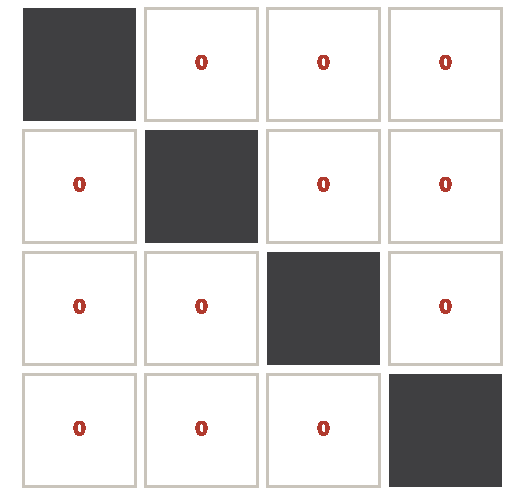
\includegraphics[width=0.8\textwidth]{figs/fig_sextuples.pdf}\\[2mm]
    {\color{faded}\scriptsize four candidate bases on one pair; every cross count is zero}
  \end{column}
  \end{columns}
\end{frame}

% ---------------------------------------------------------------- 14 what it means
\begin{frame}{What it means for quantum information}
  \vspace{2mm}
  {\footnotesize\color{faded} Four statements that survive a check against primary sources; the
  preprint itself makes no quantum-information claim.}

  \vspace{2mm}
  {\footnotesize
  \begin{description}
    \item[Tomography.] A six-level state has thirty-five real parameters and one orthonormal basis
      fixes five, so seven settings is the minimum. A complete MUB set is the error-minimising
      choice among seven-setting schemes. There are three MUBs in $\C^6$, so three bases fix fifteen
      of the thirty-five.

    \vspace{1.8mm}
    \item[Uncertainty.] The strong state-independent bound sums over a \emph{complete} MUB set, which
      needs seven bases here. With three, only the pairwise bound survives:
      $\tfrac1L\sum H\ge\tfrac12\log_2 6=1.292$ bits.

    \vspace{1.8mm}
    \item[Key distribution, unharmed.] The six-dimensional analogue of the six-state protocol would
      be a seven-MUB protocol, so it cannot exist. Ordinary qudit QKD is untouched: the two-basis
      protocol still tolerates about $22.5\%$ error at $d=6$.

    \vspace{1.8mm}
    \item[A negative result.] Nothing is enabled. Capacities that do not count MUBs --- dense coding
      at $2\log_2 6=5.17$ bits per six-level system, for instance --- are unchanged.
  \end{description}}
\end{frame}

\begin{frame}{Where this leaves the problem}
  \vspace{2mm}
  \begin{columns}[T]
  \begin{column}{0.48\textwidth}
    {\color{ox}\scshape what is settled}\\[1.5mm]
    No four mutually unbiased bases in $\C^6$, conditional on one documented run. No admissible
    vector for any decided triple. The covering step reproduced from scratch, byte-identical.
  \end{column}
  \begin{column}{0.48\textwidth}
    {\color{ox}\scshape what is not}\\[1.5mm]
    A small independent checker for the record stream. Outward-rounded arithmetic, which would
    delete the compiler dependence. A control in $\C^4$, where the same pipeline must fail. The
    Lean assembly is conditional and stops at $N(6)\le5$.
  \end{column}
  \end{columns}

  \vspace{6mm}
  \begin{center}
    {\color{ox}\rule{22mm}{1.2pt}}\\[3mm]
    {\normalsize\itshape The claim worth defending is not the number. It is that a finite,\\
    checkable object can carry an exclusion over a torus of phases ---\\
    and that we can say exactly how much of it is checked.}
  \end{center}
\end{frame}

\end{document}
